% This is LLNCS.DEM the demonstration file of
% the LaTeX macro package from Springer-Verlag
% for Lecture Notes in Computer Science,
% version 2.4 for LaTeX2e as of 16. April 2010
%
\documentclass{llncs}
%
\usepackage[portuguese]{babel}
\usepackage[utf8]{inputenc}
\usepackage{makeidx}  % allows for indexgeneration
\usepackage{graphicx}

%

\begin{document}

%
\frontmatter          % for the preliminaries
%
\pagestyle{headings}  % switches on printing of running heads
%
\title{Ano Escolar}
\subtitle{Resolução de Problemas de Otimização utilizando\\
Programação em Lógica com Restrições}
%
\titlerunning{Ano Escolar}  
%
%
%
\author{José Oliveira (up201406208) e Manuel Gomes (up201402679)}
\authorrunning{José Oliveira e Manuel Gomes}
%
\institute{FEUP-PLOG, Turma 3MIEIC3, Grupo AnoEscolar3}

\maketitle              % typeset the title of the contribution

\begin{abstract} %
No âmbito da unidade curricular de Programação em Lógica desenvolveu-se um programa capaz de gerar a calendarização das atividades avaliativas de uma turma, recorrendo-se à Programação em Lógica com Restrições com auxílio do software \textbf{\textit{SICStus Prolog}}.
Com efeito, e tendo-se em conta as várias restrições impostas para se gerar uma possível solução do problema, implementaram-se vários predicados de forma a se construir um programa o mais eficiente possível.
Através da manipulação dos vários predicados construidos, assim como os pertencentes ao \textbf{\textit{SICStus Prolog}}, conseguiu-se não só resolver o problema em específico, mas também de uma forma alargada, com calendarização de várias turmas em simultâneo.
\\\\
\textbf{Palavras-chave: }Prolog, Restrições, Ano Escolar

\end{abstract}
%
\section{Introdução}
No âmbito da unidade curricular de Programação em Lógica pretende-se desenvolver um programa capaz de gerar a calendarização das atividades avaliativas de uma turma, recorrendo-se à Programação em Lógica com Restrições com auxílio do software \textbf{\textit{SICStus Prolog}}.
Este problema consiste na calendarização de um período escolar escolar de uma turma mediante diversas restrições ao nível dos trabalhos de casa (TPCs) assim como dos testes. Por outro lado pretende-se que a solução seja eficiente, pelo que se pretende que a mesma seja extensível a mais do que uma turma, assim como não só a uma variada duração do período escolar, como também diferentes valores para as restrições pretendidas. 
O presente artigo expõe a estratégia utilizada para resolução do problema, assim como os resultados com ela obtidos.


\section{Descrição do Problema}
O problema em análise é referente à calendarização de um período escolar, com agendamento dos trabalhos de casa (TPC), assim como as datas dos testes. Para resolução do mesmo são implementadas as seguintes restrições:
\begin{enumerate}
	\item Em pelo menos um dia por semana, que deve ser o mesmo ao longo do período, não pode haver TPC;
	\item Cada dia não pode ter TPC em mais do que \textit{NumMaxTPCDay} disciplinas;
	\item Em cada disciplina só pode haver TPC no máximo em metade das aulas;
	\item Cada disciplina tem 2 testes por período de aulas, que decorrem num conjunto de semanas específico (mais ou menos a meio e no fim do período);
	\item Os estudantes não podem ter mais do que \textit{NumMaxTestsWeek} testes per semana);
	\item Os estudantes não podem ter mais do que um teste em dias consecutivos;
	\item Os testes realizados pelas diferentes turmas a uma mesma disciplina devem ser o mais próximos possível.
	
Deve ser possível resolver o problema como um problema de satisfação de restrições, de modo a que seja possível resolver problemas desta classe com diferentes parâmetros, isto é, fazendo variar o número de turmas e disciplinas, horários, número máximo de TPC por disciplina e por dia, entre outros.

\end{enumerate}

\section{Abordagem}

Por forma a se desenvolver o método o mais adequado à resolução do problema, começou-se por tentar modelar o calendário de um ano escolar como um problema de restrições. Findo este processo, procurou-se entender as variáveis de decisão a utilizar, assim como a forma mais correta de restringir as mesmas, de modo a tornar a solução o mais eficiente quanto possível.

\subsection{Variáveis de Decisão}

Para estruturação do problema em análise, e assim para uma mais fácil legibilidade do mesmo, optou-se por construir para cada turma uma lista de listas, sendo que cada lista corresponde a uma diferente disciplina.
Cada lista de uma disciplina possui um identificador da disciplina, assim como uma lista com os TPC's e outra com os Testes, de tamanho igual ao número de dias do do período. As variáveis de decisão presentes em cada uma das listas podem assumir o valor de 0 (\textit{falso}), ou de 1 (\textit{verdadeiro}), caso se encontre uma ocorrência de um TPC ou teste.

\subsection{Restrições}
\begin{enumerate}

	\item \textbf{Em pelo menos um dia por semana, que deve ser o mesmo ao longo do período, não pode haver TPC:}\\\\	               
		De modo a se implementar esta restrição, foi desenvolvido o predicado \textit{freeTPC(+FreeTPCDay, +Class)}, que recebe o dia em que não deve haver TPC, podendo o mesmo oscilar entre 1 e 5 (representativo de um dia da semana), percorrendo a lista de TPC's de cada uma das disciplinas e instanciando as variáveis de decisão correspondentes com o valor de 0 (\textit{falso}).
		\\
	\item \textbf{Cada dia não pode ter TPC em mais do que \textit{NumMaxTPCDay} disciplinas:}\\\\	               
		Para esta restrição foi implementado o predicao \textit{maxNumTPCDay(+Day, +Days, +Class, +NumMaxTPCDay)}, que recebe o número máximo de TPC's para cada dia representado por \textit{NumMaxTPCDay}. São percorridas as listas de TPC's de cada disciplina e criadas uma lista para cada dia com   as variáveis de decisão correspondentes. Por fim, é colocada a restrição de que o somatório de cada uma dessas listas deve ser menor ou igual a \textit{NumMaxTPCDay}.
		\\
	\item \textbf{Em cada disciplina só pode haver TPC no máximo em metade das aulas:}\\\\	               
		Nesta restrição foi implementado o predicado \textit{maxTPCPeriod(+Days, +RatioTPC, +Schedule, +Class)}, o qual recebe a percentagem de máxima das aulas em que pode haver TPC. De modo a implementar esta restrição é determinado primeiramente o número de aulas de cada disciplina ao longo do período escolar, a partir do qual, e utilizando-se \textit{RatioTPC}, é calculado o número de dias máximo para cada disciplina em que pode haver TPC. Por fim é restringindo-se o somatório da lista de TPC's de cada disciplina, de modo a que este seja menor ou igual ao número máximo de TPC's por período respetivo.
		\\
	\item \textbf{ Cada disciplina tem dois testes por período de aulas, que decorrem num conjunto de semanas específico (mais ou menos a meio e no fim do período):}\\\\	               
		Para resolução desta restrição foram utilizados dois predicados. Para a restrição de haverem dois testes por período de aulas foi utilizado o predicado \textit{twoTestsDisciplinePeriod(+Class)}, o qual para cada lista de testes de cada disciplina, restringe o valor da soma dos elementos para que seja igual a 2. Por outro lado, e de modo a solucionar a segunda parte da restrição, foi implementada a restrição \textit{twoDifferentTestMoments(+StartFirstTestMoment, +TestMomentDuration, +StartSecondTestMoment, +Class}, a qual começa primeiro por determinar o começo e duração de cada um dos dois momentos de avaliação. Para tal, é obtido o quociente entre o número de dias correspondente à duração do período escolar e o valor de 4. Este valor de quociente não só corresponderá à duração de cada momento de avaliação, assim como também será utilizado para o cálculo do começo de cada avaliação, sendo que o primeiro período de avaliação ocorrerá durante o segundo quarto do período e o segundo momento de avaliação o último quarto do período.
		\\
	\item \textbf{Os estudantes não podem ter mais do que \textit{NumMaxTestsWeek} testes per semana):}\\\\	               
		De modo a se implementar esta restrição foi desenvolvido o predicado \textit{maxTestsPerWeek(+Day, +Days, +NumMaxTestsWeek, +Class)}, o qual recebe o número máximo possível de testes por semana \textit{NumMaxTestsWeek}. Neste predicado é gerada uma lista para cada semana, com as variáveis de decisão representativas dos dias, a partir de cada uma das listas de testes de cada disciplina. Por fim, restringe-se a que o somatório de cada uma destas listas (semanas) seja menor ou igual a \textit{NumMaxTestsWeek}.
		\\
	\item \textbf{Os estudantes não podem ter mais do que um teste em dias consecutivos:}\\\\	               
		Para a implementação deste predicado foi desenvolvido o predicado \textit{testsConsecutiveDays(+Day, +Days, +Class)}, o qual em cada iteração cria duas listas, cada uma das quais com as variáveis de decisão correspondentes a dois dias diferentes e consecutivos, até que todos os dias do período sejam percorridos.  Por fim é restringido o somatório das duas para que seja menor ou igual a um. Note-se que caso os dois dias consecutivos se tratem de Sexta-feira e Segunda-feira, será possível ter teste nestes dois dias, uma vez que existe o fim-de-semana entre os mesmos.
		\\
	\item \textbf{Os testes realizados pelas diferentes turmas a uma mesma disciplina devem ser o mais próximos possível:}\\\\	               
	Para esta restrição é usado o predicado \textit{testsCloseDays(+Classes, +Test1, +Test2)}, o qual para cada diferente disciplina, tenta restringir a diferença de dias de um teste de uma mesma disciplina, para turmas diferentes, sendo esse valor representado por \textit{Test1}	e \textit{Test2}. Estes valores serão depois minimizados através da estratégia de etiquetagem utilizada com o uso da opção \textit{minimize}.	\\
		
	

\end{enumerate} 

\subsection{ Função de Avaliação}
Para testar e avaliar a solução obtida é usado o predicado \textit{run(+Days, +FreeTPCDay, +NumMaxTPCDay, +RatioTPC, +NumMaxTestsWeek, +ClassResult)}, o qual verifica se o tempo de execução do programa. Por outro lado é neste predicado que é efetuada a restrição que minimiza o tempo entre testes de várias turmas de uma mesma disciplina.

\subsection{Estratégia de Pesquisa}
Em termos de processo de etiquetagem foi usado o predicado \textit{labeling([ffc, down, minimize(Test1), minimize(Test2), step, time\_out(120000, \_], Result)}, em que \textit{Result} corresponde a todas as varáveis a serem instanciadas.
É utilizada a estratégia de \textit{first-fail} através de \textit{ffc} em que as variáveis que participam  em mais restrições são etiquetadas primeiro. Por outro lado, através de \textit{down} os elementos de domínio são etiquetados por ordem descendente do seu intervalo de domínio.\\
Em relação aos \textit{minimize(Test1)} e \textit{minimize(Test2)}, os mesmos são usados de modo a que a solução obtida para as datas dos testes, seja a mais próxima possível para testes de uma mesma disciplina.
Por fim, a estratégia de \textit{branching} utilizada foi a estratégia padrão do predicado \textit{labeling}, ou seja, foi utilizada a opção \textit{step}.






\section{Visualização da Solução}
Para se efetuar a visualização do resultado é utilizado o predicado \textit{displayResults(+Days, +Schedules, +ClassResults)}, o qual recebe as listas com os diferentes horários, assim como os resultados para as distribuições dos TPC's e testes para cada turma.\\
Este predicado começa por imprimir em modo de texto o horário da turma respetiva através do predicado \textit{displaySchedule(+Day, +Schedule)}, o qual utiliza a variável \textit{Day} instanciada com o valor zero, de modo a ser usada para que se possa imprimir o nome do dia da semana corretamente. Assim, e de forma recursiva, até a lista \textit{Schedule} estar vazia, uma nova variável é instanciada sendo igual ao  valor de \textit{Day}, acrescido de uma unidade.\\

\begin{figure}
\centering
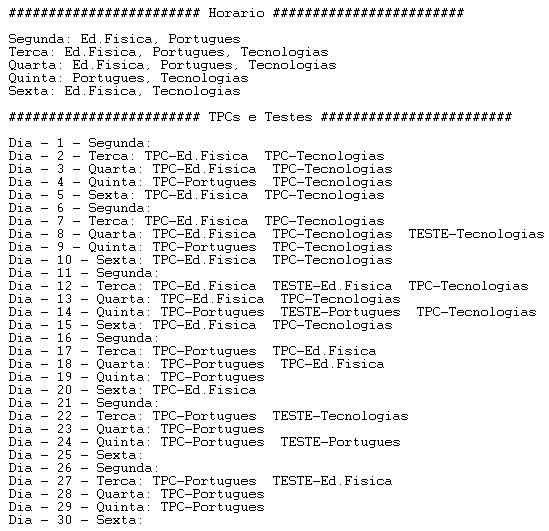
\includegraphics[scale=0.8]{display.png}
\caption{Exemplo de um resultado de visualização para uma turma}
\end{figure}

Por fim, é usado o predicado \textit{displayTPCsAndTests(+StatingDay, +EndDay, +ClassResult)}, o qual recebendo os dias inicial e final do período, imprime a calendarização de TPC's e testes para cada turma. Neste predicado, para cada dia do período, é percorrida a lista de disciplinas, sendo usado o predicado \textit{nth0/3} de modo a que, usando o dia do período em questão como índice para as respetivas listas de TPC's e testes, se verifica se para aquele determinado dia existe algum destas ocorrências. Em caso afirmativo é então imprimido o nome da disciplina seguido do tipo de ocorrência.

\section{Resultados}
Para a obtenção dos resultados, foram efetuadas diversas simulações, com diferentes valores de turmas, disciplinas, assim como duração do período escolar. Deste modo apresentam-se os resultados obtido para 3 e 6 turmas com 3 disciplinas, e fazendo-se variar a duração do período escolar.

\begin{figure}
\centering
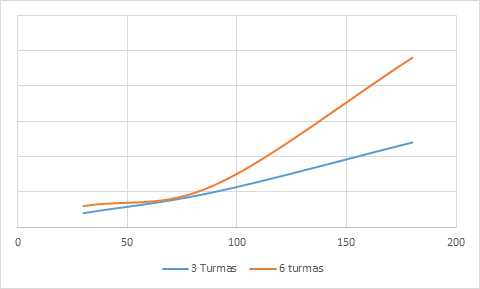
\includegraphics[scale=0.8]{grafico1.png}
\caption{Resultados obtidos para 3 turmas}
\end{figure}

Como seria de esperar, com o aumento da duração do período escolar, assim como do número de turmas o processamento do resultado é mais demorado. No entanto, verifica-se que com o aumento do número de turmas,  o aumento do tempo de processamento é mais rápido do que com o aumento do número de turmas.\\
Por outro lado, testou-se também com um número variável de disciplinas, tendo-se experimentado o valor de 10 disciplinas. No entanto, não foi possível obter qualquer solulão dentro do tempo de \textit{time\_out} de 120 segundos, pelo que assim se pode verificar que esta variável, a par do número de turmas, são as que mais influênciam a rapidez de obtenção de uma solução para o programa desenvolvido.


\section{Conclusões e Trabalho Futuro}
Com a realização deste trabalho verifica-se que a linguagem \textit{Prolog}, mais especificamente os seus módulos de resolução com restrições, é bastante poderosa para resolver uma ampla variedade de problemas de decisão e/ou otimização, tal como fui possível constatar com o seu predicado \textit{labeling}.
\\Em relação à solução obtida para o problema proposto, consideramos que a mesma atingiu de forma satisfatória os objetivos propostos, implementando não só todas as restrições pedidas, como também apresentando os resultados de forma eficiente.
\\No que diz aos resultados obtidos, verifica-se que o principal fator que leva a um maior tempo de processamento de uma solução é o aumento do número de disciplinas e/ou turmas, pelo que seria neste âmbito que se poderia tentar tornar a solução ainda mais eficiente. Por outro lado, a implementação de novas restrições de forma a tornar o programa desenvolvido ainda mais completo, seria um outro ponto poder ser desenvolvido  em iterações futuras.




\begin{thebibliography}{5}
%
\bibitem {url} 
Vários autores, SWI-Prolog,\\
\url{http://www.swi-prolog.org}\\
\bibitem {url} 
Vários autores, The Prolog Library,\\
\url{https://sicstus.sics.se/sicstus/docs/4.3.0/html/sicstus/The-Prolog-Library.html}\\
\bibitem {url} 
Pierre Deransart, AbdelAli Ed-Dbali, Laurent Cervoni, Prolog The Standard: Reference Manual, Springer, 2007\\

\end{thebibliography}
\clearpage

\section*{Anexo}
A totalidade do código desenvolvido encontra-se na pasta \textit{codigo}.


\end{document}
